\documentclass[a4paper,12pt,hidelinks]{report}

%%Pacchetti utili anche se non necessari

\usepackage{amsfonts}
\usepackage{amsmath}
\usepackage{latexsym}
\usepackage{tabularx}
\usepackage[italian]{babel}
\usepackage[bookmarks=true]{hyperref}
\usepackage{url}
% \usepackage{subfigure}
\usepackage{epstopdf}
\usepackage[utf8]{inputenc}
% \usepackage[utf8x]{inputenc}
\usepackage{listings}
\usepackage{graphicx}
%-------------------------------------------

% \title{Progettazione sito web\\ ''B\&B La Vecchia Posta''}
% \author{Daniele Di Pompeo \\mat. 226766}
% \annoaccademico{2013-2014}
\begin{document}
  \begin{titlepage}
    \begin{center}
    % Upper part of the page
      
\includegraphics[width=0.5\textwidth,keepaspectratio=true]{../img/logo}\\[1cm]    
      \textsc{\LARGE Mappa del sito}\\[0.6cm]
      \textsc{\LARGE  progetto:\\[0.5cm] ``B\&B La Vecchia Posta''}\\ [2.0cm]

    % Author and supervisor
      \begin{minipage}{0.8\textwidth}
	\begin{flushleft} \large
	  \emph{Autore:} Daniele Di Pompeo \\[0.5cm]
	  \emph{Versione documento: 1.0}\\[0.5cm]
	  \emph{Data emissione del documento: \today}\\[0.5cm]
	\end{flushleft}
      \end{minipage}
    \end{center}
  \end{titlepage}

\begin{figure}[h!]%
    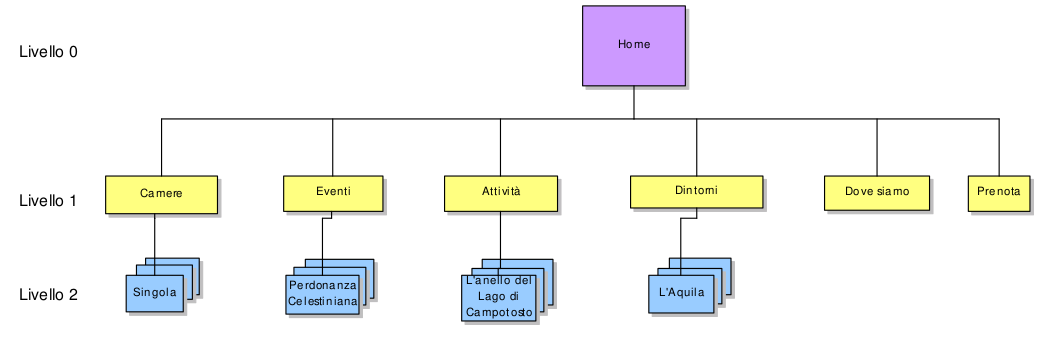
\includegraphics[width=1\textwidth,keepaspectratio=true]{../img/sitemap}
    \centering
    \caption{Mappa del sito}%
    \label{fig:sitemap}%
\end{figure}

Vengono riportati di seguito i possibili percorsi da una pagina ad un'altra raggruppandoli per sezioni.

\end{document}          
